%%
%% This is file `tikzposter-template.tex',
%% generated with the docstrip utility.
%%
%% The original source files were:
%%
%% tikzposter.dtx  (with options: `tikzposter-template.tex')
%%
%% This is a generated file.
%%
%% Copyright (C) 2014 by Pascal Richter, Elena Botoeva, Richard Barnard, and Dirk Surmann
%%
%% This file may be distributed and/or modified under the
%% conditions of the LaTeX Project Public License, either
%% version 2.0 of this license or (at your option) any later
%% version. The latest version of this license is in:
%%
%% http://www.latex-project.org/lppl.txt
%%
%% and version 2.0 or later is part of all distributions of
%% LaTeX version 2013/12/01 or later.
%%


\documentclass{tikzposter} %Options for format can be included here

\usepackage{todonotes}
\usepackage{epstopdf}
\usepackage[tikz]{bclogo}
\usepackage{lipsum}
\usepackage{amsmath}
\usepackage{makecell}
\usepackage{booktabs}
\usepackage{longtable}
\usepackage[absolute]{textpos}
\usepackage[it]{subfigure}
\usepackage{graphicx}
\usepackage{cmbright}
%\usepackage[default]{cantarell}
%\usepackage{avant}
%\usepackage[math]{iwona}
\usepackage[math]{kurier}
\usepackage[T1]{fontenc}


%% add your packages here
\usepackage{hyperref}
% for random text
\usepackage{lipsum}
\usepackage[english]{babel}
\usepackage[pangram]{blindtext}

\colorlet{backgroundcolor}{blue!10}

 % Title, Author, Institute
\title{Traffic Flow Prediction In a U.S. Metropolis}
\author{Jingbao Luo}
\institute{Nanjing University of Science and Technology, China \\
}
%\titlegraphic{logos/tulip-logo.eps}

%Choose Layout
\usetheme{Wave}

%\definebackgroundstyle{samplebackgroundstyle}{
%\draw[inner sep=0pt, line width=0pt, color=red, fill=backgroundcolor!30!black]
%(bottomleft) rectangle (topright);
%}
%
%\colorlet{backgroundcolor}{blue!10}

\begin{document}


\colorlet{blocktitlebgcolor}{blue!23}

 % Title block with title, author, logo, etc.
\maketitle

\begin{columns}
 % FIRST column
\column{0.5}% Width set relative to text width

%%%%%%%%%% -------------------------------------------------------------------- %%%%%%%%%%
 %\block{Main Objectives}{
%  	      	\begin{enumerate}
%  	      	\item Formalise research problem by extending \emph{outlying aspects mining}
%  	      	\item Proposed \emph{GOAM} algorithm is to solve research problem
%  	      	\item Utilise pruning strategies to reduce time complexity
%  	      	\end{enumerate}
%%  	      \end{minipage}
%}
%%%%%%%%%% -------------------------------------------------------------------- %%%%%%%%%%


%%%%%%%%%% -------------------------------------------------------------------- %%%%%%%%%%
\block{Problem Definition}{
  \begin{description}
    \item The March edition of the 2022 Tabular Playground Series
    is a prediction project about time series data.
    We'll forecast twelve-hours of traffic flow in a major U.S. 
    metropolitan area. Time, space, and directional features 
    give us the chance to 
    model interactions across a network of roadways.
  \end{description}
  \vspace{.5cm}
  \begin{center}
    \begin{tabular}{ c | c | c }
      \toprule
        % after \\: \hline or \cline{col1-col2} \cline{col3-col4} ...
      File    &Description      & Attribution       \\
      \midrule
      train.csv       &  \makecell{traffic congestion from April\\through September of 1991}   &  \makecell{row\_id,time,x,y,\\direction,congestion}       \\
      \midrule
      test.csv       & \makecell{hourly predictions \\on the day of 1991-09-30}   &\makecell{row\_id,time,x,y,\\direction}     \\
      \bottomrule
    \end{tabular}
  \end{center}
}
%%%%%%%%%% -------------------------------------------------------------------- %%%%%%%%%%


%%%%%%%%%% -------------------------------------------------------------------- %%%%%%%%%%
\block{Data Processing}
{
\begin{itemize}
    \item Split Time data
    \item Merge x,y,row\_id
\end{itemize}
}
%%%%%%%%%% -------------------------------------------------------------------- %%%%%%%%%%


%%%%%%%%%% -------------------------------------------------------------------- %%%%%%%%%%

%\note{Note with default behavior}

%\note[targetoffsetx=12cm, targetoffsety=-1cm, angle=20, rotate=25]
%{Note \\ offset and rotated}

 % First column - second block


%%%%%%%%%% -------------------------------------------------------------------- %%%%%%%%%%
\block{Data Description}{		
\begin{description}
  \item [Congestion]
\end{description}
\vspace{.2cm}
\begin{center}

    \includegraphics{./figure/congestion.eps}
\end{center}
\begin{description}
  \item [The effect of hour on congestion group by road ]
\end{description}
\vspace{.2cm}
\begin{center}

    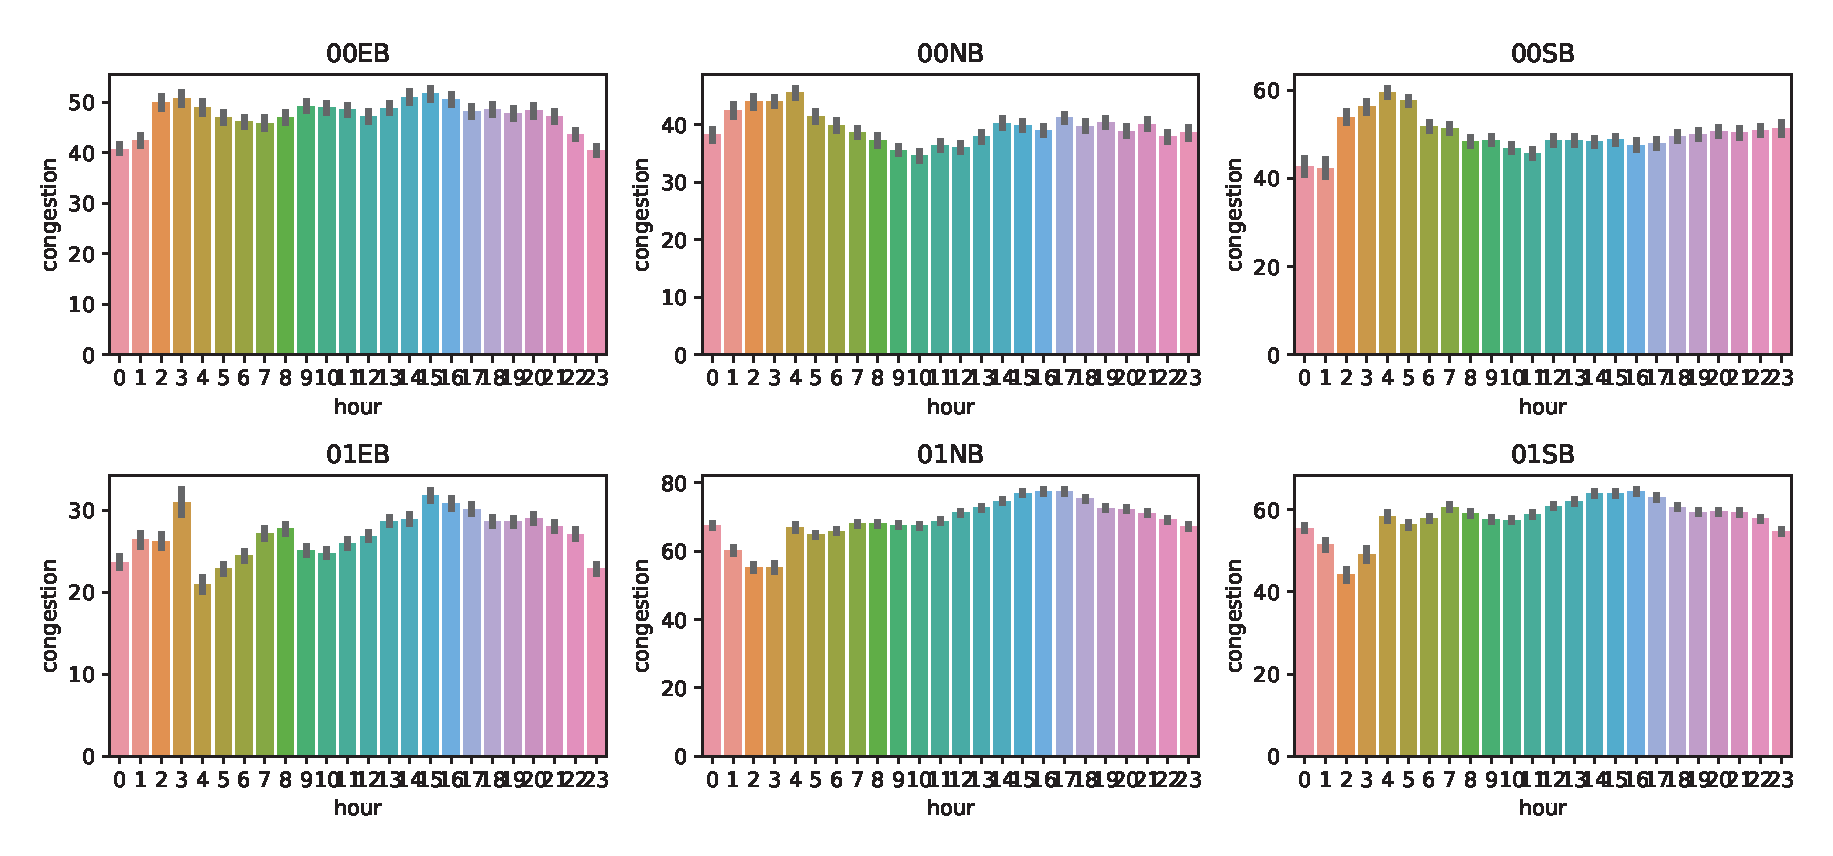
\includegraphics{./figure/road.eps}
\end{center}
\begin{description}
  \item [The effect of day on congestion group by month ]
\end{description}
\vspace{.2cm}
\begin{center}
    \includegraphics[scale=0.8]{./figure/day.eps}
\end{center}
}
%%%%%%%%%% -------------------------------------------------------------------- %%%%%%%%%%


% SECOND column
\column{0.5}
 %Second column with first block's top edge aligned with with previous column's top.

%%%%%%%%%% -------------------------------------------------------------------- %%%%%%%%%%
\block{ Model Train and Evaluation}{
  \begin{itemize}
    
    \item Data feature
    \vspace{.3cm}
      \begin{description}
        \item road,hour,month,weekday,minute,period,is\_weekend,is\_Friday,is\_Monday,
        Month\_start,Month\_end
      \end{description}
    \vspace{.3cm}
    \item By using sklearn.package ,split train data and evaluation data
    \vspace{.3cm}
    \item Use ligthgbm model
\end{itemize}
\vspace{.5cm}
\begin{center}
  \includegraphics[scale=2]{./figure/feature_importance.eps}
\end{center}
\begin{description}
  \item[Evaluation result]
\end{description}
\vspace{.5cm}
\begin{center}
  \begin{tabular}{p{14cm}p{14cm}}
    \hline
      Index & Result  \\
    \hline
      explained\_variance\_score   & 0.7277243544483329    \\
      mean\_absolute\_error&  6.167491947603395 \\
      r2\_score & 0.7277251135484366  \\
    \hline
  \end{tabular}
\end{center}

}
%%%%%%%%%% -------------------------------------------------------------------- %%%%%%%%%%
% Second column - first block


%%%%%%%%%% -------------------------------------------------------------------- %%%%%%%%%%
\block[titleleft]{Result}
{
\begin{description}
  	\item[Prediction Result] 
\end{description}
\vspace{.5cm}
\begin{center}
  \begin{tabular}{p{6cm}p{6cm}p{6cm}p{6cm}}
    \hline
      Row\_id & Congestion  &  Row\_id & Congestion \\
    \hline
    848835 & 47 & 848836 & 33\\
    848837 & 39 & 848838 & 54\\
    848839 & 64 & 848840 & 23\\
    848841 & 28 & 848842 & 70\\
    848843 & 25 & 848844 & 47\\
    848845 & 46 & 848846 & 25\\
    848847 & 69 & 848848 & 60\\
    \hline
    \end{tabular}
\end{center}
}
%%%%%%%%%% -------------------------------------------------------------------- %%%%%%%%%%


% Second column - second block
%%%%%%%%%% -------------------------------------------------------------------- %%%%%%%%%%
\block[titlewidthscale=1, bodywidthscale=1]
{Conclusion}
{
  This experiment simply obtains the eigenvalues from the time
   data and uses the 
  lightgbm model for training, 
  but does not optimize the model.
}
%%%%%%%%%% -------------------------------------------------------------------- %%%%%%%%%%


% Bottomblock
%%%%%%%%%% -------------------------------------------------------------------- %%%%%%%%%%


%\note[targetoffsetx=8cm, targetoffsety=-10cm,rotate=0,angle=180,radius=8cm,width=.46\textwidth,innersep=.1cm]{
%Acknowledgement
%}

%\block[titlewidthscale=0.9, bodywidthscale=0.9]
%{Acknowledgement}{
%}
%%%%%%%%%% -------------------------------------------------------------------- %%%%%%%%%%

\end{columns}


%%%%%%%%%% -------------------------------------------------------------------- %%%%%%%%%%
%[titleleft, titleoffsetx=2em, titleoffsety=1em, bodyoffsetx=2em,%
%roundedcorners=10, linewidth=0mm, titlewidthscale=0.7,%
%bodywidthscale=0.9, titlecenter]

%\colorlet{noteframecolor}{blue!20}
\colorlet{notebgcolor}{blue!20}
\colorlet{notefrcolor}{blue!20}
\note[targetoffsetx=-13cm, targetoffsety=-12cm,rotate=0,angle=180,radius=8cm,width=.96\textwidth,innersep=.4cm]
{
\begin{minipage}{0.3\linewidth}
\centering
\includegraphics[width=24cm]{./graphics/logos/tulip-wordmark.eps}
\end{minipage}
\begin{minipage}{0.7\linewidth}
{ \centering
  The March edition of the 2022 Tabular Playground Series on Kaggle Competition
}
\end{minipage}
}
%%%%%%%%%% -------------------------------------------------------------------- %%%%%%%%%%


\end{document}

%\endinput
%%
%% End of file `tikzposter-template.tex'.
